\documentclass[11pt,a4paper]{article}
\usepackage[utf8]{inputenc}
\usepackage{color}
\usepackage{enumerate}
\usepackage{fancyhdr}
\usepackage{minted}
\usepackage{graphicx}
\usepackage{array}
\usepackage{hyperref}
\usepackage{amssymb}
\usepackage[spanish]{babel}
\usepackage[spanish]{algorithm2e}

\setlength{\oddsidemargin}{18pt}
\setlength{\headheight}{14pt}
\setlength{\textheight}{609pt}
\setlength{\marginparsep}{11pt}
\setlength{\footskip}{30pt}
\hoffset = 0pt
\voffset = 0pt
\setlength{\topmargin}{0pt}
\setlength{\headsep}{25pt}
\setlength{\textwidth}{424pt}
\setlength{\marginparwidth}{54pt}
\setlength{\marginparpush}{5pt}
\paperwidth = 597pt
\paperheight = 845pt

\pagestyle{fancy}
\fancyhead[LO]{\textcolor[rgb]{0,0,0}{Grado en Ingeniería Informática}}
\fancyhead[RO]{\textcolor[rgb]{0.2,0.2,0.9}{Algorítmica, Curso 2015-2016}}

\hypersetup{
	colorlinks,
	citecolor=black,
	filecolor=black,
	linkcolor=black,
	urlcolor=black
}

\begin{document}

	\begin{titlepage}

		\centering

		\begin{figure}[h]

			\centering
			
\includegraphics[width=0.6\textwidth]{logo-ugr.png}
			
		\end{figure}

		\vspace{1cm}

		{\scshape\LARGE Universidad de Granada}

		\vspace{1cm}

		{\LARGE Algorítmica}

		\vspace{1cm}

		{\huge\bfseries\textit{Algoritmos Greedy, parte 2}}

		\vspace{1cm}

		{\itshape\large 
		Laura Calle Caraballo \\
		Cristina María Garrido López \\
		Germán González Almagro \\
		Javier León Palomares \\
		Antonio Manuel Milán Jiménez}

		\vfill

		{\Large\today}

	\end{titlepage}

\newpage

	\tableofcontents

\newpage

	\section{Introducción.}

		\par
		El objetivo de esta práctica es el estudio de los algoritmos de tipo \textit{Greedy} aplicados particularmente al problema del viajante de comercio. Para ello, hemos implementado tres variantes según el criterio utilizado a la hora de construir soluciones y las hemos comparado según su grado de desviación respecto a las soluciones óptimas.

	\section{Descripción del problema.}

		\par
		El problema del viajante de comercio, también llamado \textit{TSP} por sus siglas en inglés, es conocido desde el siglo XIX y fue planteado en su forma general en la década de 1930; desde entonces, es uno de los problemas más estudiados en optimización. Su complejidad hace computacionalmente muy costosa una solución mediante fuerza bruta. Por ello, se han ido creando una serie de métodos que obtienen resultados válidos según la situación: soluciones exactas para dimensiones pequeñas, aproximadas para dimensiones más grandes o particularizaciones del problema donde se pueda emplear una aproximación mejor.

		\par
		La pregunta que busca responder este problema es la siguiente: \textit{``Considerando un conjunto de ciudades y las distancias entre ellas dos a dos, ¿cuál es el camino más corto que pasa por todas ellas una única vez y retorna al origen?''}

		\par
		En términos de grafos esto significa que, a partir de un grafo ponderado, conexo y no dirigido, debemos encontrar el circuito hamiltoniano de menor peso.

	\section{Resolución.}

		\par
		Se han diseñado tres algoritmos \textit{Greedy} para encontrar soluciones al problema en diferentes instancias de prueba; la diferencia que existe entre ellos es la estrategia de elección de la siguiente ciudad a incluir en el camino (Función Selección): el vecino más cercano, la inserción más económica o la inserción radial.

		\par
		Los elementos comunes a los tres algoritmos son los siguientes:

		\begin{itemize}

			\item
			Conjunto de Candidatos: ciudades de la instancia a evaluar.
			\item
			Conjunto de Seleccionados: ciudades ya incluidas en el circuito.
			\item
			Función Solución: todas las ciudades forman parte del circuito.
			\item
			Función de Factibilidad: se puede o no completar el circuito a partir de las ciudades ya elegidas.
			\item
			Función Objetivo: el circuito y su coste.

		\end{itemize}

\newpage

	\section{Estrategia del vecino más cercano (O($n^3$)).}

		\par
		La estrategia del vecino más cercano es la forma más intuitiva de buscar el recorrido más corto: a partir de una ciudad, buscamos la más cercana que esté conectada a ella sin formar ya parte del circuito; a continuación, nos situamos sobre esta nueva ciudad y repetimos el proceso hasta que todas las ciudades hayan sido visitadas, construyendo un circuito hamiltoniano de forma secuencial.

		\par
		Adicionalmente, comenzaremos el algoritmo desde todas las ciudades y nos quedaremos con el circuito más corto de todos los obtenidos.

		\par
		La correspondiente Función Selección consiste en escoger la ciudad cuya distancia a la última añadida al circuito parcial sea mínima.

		\subsection{Pseudocódigo.}

			\par
			A continuación se muestra el pseudocódigo del algoritmo:

			\vspace{2mm}

			\begin{algorithm}[H]

				\textbf{function} Greedy(conjuntoCiudades);

				costeMejorCircuito $\longleftarrow \infty$\;

				\Begin{

					\For{$ciudadInicial \in$ conjuntoCiudades}{

						ciudadActual $\longleftarrow$ ciudadInicial\;
						circuito $\longleftarrow$ ciudadInicial\;
						costeCircuito $\longleftarrow 0$\;

						\For{$i = 2$ \textbf{to} $n$}{

							mejorVecino $\longleftarrow$ EncontrarVecinoMasCercano(ciudadActual)\;
							circuito $\longleftarrow$ circuito $\cup$ mejorVecino\;
							costeCircuito $\longleftarrow$ costeCircuito $+$ costeMejorVecino\;
							ciudadActual $\longleftarrow$ mejorVecino\;

						}

						cerrar circuito con ciudadInicial\;
						actualizar costeCircuito\;

						\If{costeCircuito $<$ costeMejorCircuito}{

							guardar circuito y actualizar costeMejorCircuito\;

						}

					}

						\KwRet circuito, costeMejorCircuito\;

				}

			\end{algorithm}

\newpage

		\subsection{Resultados.}

			\begin{figure}[h]

				\centering

				\begin{tabular}{| >{\centering\arraybackslash}m{1in} | >{\centering\arraybackslash}m{1in} | >{\centering\arraybackslash}m{1in} |}

					\hline
					\textbf{Conjunto de datos} & \textbf{Óptimo} & \textbf{Resultado} \\
					\hline
					att48 & 33524 & 37897 \\
					\hline
					berlin52 & 7542 & 8181 \\
					\hline
					eil51 & 426 & 482 \\
					\hline
					eil76 & 538 & 608 \\
					\hline
					eil101 & 629 & 746 \\
					\hline
					gr96 & 512 & 621 \\
					\hline
					gr120 & 1666 & 1836 \\
					\hline
					lin105 & 14379 & 16935 \\
					\hline
					pr76 & 108159 & 130921 \\
					\hline
					st70 & 675 & 796 \\
					\hline

				\end{tabular}
				\caption{Resultados obtenidos por la heurística del vecino más cercano.}

			\end{figure}
	
\newpage

	\section{Estrategia de la inserción más económica (O($n^3$)).}

		\par
		La idea subyacente a esta heurística es que en cada iteración se prueba cada ciudad candidata en todas las posibles posiciones donde se podría insertar. Por ello, la Función Selección consiste en escoger, de entre las candidatas en cada momento, la ciudad cuya inserción provoque el menor aumento del coste del circuito.

		\subsection{Pseudocódigo.}

			\par
			El pseudocódigo del algoritmo es el siguiente:

			\vspace{2mm}

			\begin{algorithm}[H]

				\textbf{function} Greedy(conjuntoCiudades);

				circuito $\longleftarrow$ SolucionParcial()\;

				\Begin{

					\For{$i = 3$ \textbf{to} $n$}{

						\For{$ciudad \in$ candidatos}{

							posInsercion $\longleftarrow$ EncontrarInsercionMasEconomica($ciudad$)\;

							\If{Aumento(ciudad,posInsercion) $<$ Aumento(mejorCiudad,posMejorInsercion)}{

								posMejorInsercion $\longleftarrow$ posInsercion\;
								mejorCiudad $\longleftarrow$ ciudad\;

							}

						}

						Insertar(mejorCiudad, posMejorInsercion, circuito)\;

					}

					coste $\longleftarrow$ CalcularCoste(circuito)\;

					\KwRet circuito, coste\;

				}

			\end{algorithm}

%\newpage

		\subsection{Resultados.}

			\begin{figure}[h]

				\centering

				\begin{tabular}{| >{\centering\arraybackslash}m{1in} | >{\centering\arraybackslash}m{1in} | >{\centering\arraybackslash}m{1in} |}

					\hline
					\textbf{Conjunto de datos} & \textbf{Óptimo} & \textbf{Resultado} \\
					\hline
					att48 & 33524 & 34682 \\
					\hline
					berlin52 & 7542 & 8286 \\
					\hline
					eil51 & 426 & 454 \\
					\hline
					eil76 & 538 & 602 \\
					\hline
					eil101 & 629 & 697 \\
					\hline
					gr96 & 512 & 578 \\
					\hline
					gr120 & 1666 & 1745 \\
					\hline
					lin105 & 14379 & 16126 \\
					\hline
					pr76 & 108159 & 115546 \\
					\hline
					st70 & 675 & 741 \\
					\hline

				\end{tabular}
				\caption{Resultados obtenidos por la heurística de la inserción más económica.}

			\end{figure}

\newpage

	\section{Estrategia de inserción radial (O($n^2$)).}

		\par
		En esta heurística de cosecha propia, la idea es fijar una ciudad situada aproximadamente en el centro de todas las demás y construir un circuito parcial. Posteriormente, se tomará como mejor candidata aquella ciudad que esté más lejos de la ciudad central, insertándola en la posición que provoque el menor incremento de la longitud del circuito.
		\par
		La Función Selección asociada consiste, por tanto, en escoger en cada paso la ciudad más lejana al centro en la posición menos costosa.

		\subsection{Pseudocódigo.}

			El pseudocódigo asociado a este algoritmo se muestra a continuación:

			\vspace{2mm}

			\begin{algorithm}[H]

				\textbf{function} Greedy(conjuntoCiudades);

				circuito $\longleftarrow$ SolucionParcial()\;

				\Begin{

					ciudadCentral $\longleftarrow$ CiudadMasCercanaAlCentro()\;

					\For{$i = 3$ \textbf{to} $n$}{

						ciudadAInsertar $\longleftarrow$ CiudadMasLejana(ciudadCentral)\;

						posInsercion $\longleftarrow$ EncontrarInsercionMasEconomica(ciudadAInsertar)\;

						Insertar(ciudadAInsertar,posInsercion,circuito)\;

					}

					coste $\longleftarrow$ CalcularCoste(circuito)\;

					\KwRet circuito,coste\;

				}
			\end{algorithm}

		\subsection{Resultados.}

			\begin{figure}[h]

				\centering

				\begin{tabular}{| >{\centering\arraybackslash}m{1in} | >{\centering\arraybackslash}m{1in} | >{\centering\arraybackslash}m{1in} |}

					\hline
					\textbf{Conjunto de datos} & \textbf{Óptimo} & \textbf{Resultado} \\
					\hline
					att48 & 33524 & 65884 \\
					\hline
					berlin52 & 7542 & 12907 \\
					\hline
					eil51 & 426 & 740 \\
					\hline
					eil76 & 538 & 1083 \\
					\hline
					eil101 & 629 & 1246 \\
					\hline
					gr96 & 512 & 960 \\
					\hline
					gr120 & 1666 & 3868 \\
					\hline
					lin105 & 14379 & 32858 \\
					\hline
					pr76 & 108159 & 250946 \\
					\hline
					st70 & 675 & 1536 \\
					\hline

				\end{tabular}
				\caption{Resultados obtenidos por la heurística de inserción radial.}

			\end{figure}

\newpage

	\section{Comparación de resultados.}

		\par
		En este apartado se muestra con más claridad lo que ya se podía comprobar en secciones anteriores: la heurística que mejores resultados ha dado es la de la inserción más económica, seguida de la del vecino más cercano y de la de inserción radial.
		\par
		Es destacable, aunque de esperar, la diferencia entre las dos primeras y la inserción radial, ya que esta última es de nuestra cosecha y compite frente a dos estrategias ya consolidadas.
		\par
		Si nos centramos en las estrategias de vecino más cercano e inserción más económica, podemos observar que, en general, su rendimiento es muy bueno si consideramos su naturaleza \textit{Greedy}; en particular, y como ya comentábamos, la inserción más económica consigue a veces unos resultados especialmente competitivos.

		\subsection{Tabla comparativa de la calidad de las soluciones.}

			\begin{figure}[h]

				\centering

				\begin{tabular}{| >{\centering\arraybackslash}m{1in} | >{\centering\arraybackslash}m{1in} | >{\centering\arraybackslash}m{1in} | >{\centering\arraybackslash}m{1in} |}

					\hline
					\textbf{Conjunto de datos} & \textbf{Vecino más cercano} & \textbf{Inserción más económica} & \textbf{Inserción radial} \\
					\hline
					att48 & 13,044 & 3,454 & 96,528 \\
					\hline
					berlin52 & 8,472 & 9,865 & 71,135 \\
					\hline
					eil51 & 13,145 & 6,573 & 73,71 \\
					\hline
					eil76 & 13,011 & 11,896 & 101,301 \\
					\hline
					eil101 & 18,601 & 10,811 & 98,092 \\
					\hline
					gr96 & 21,289 & 12,891 & 87,5 \\
					\hline
					gr120 & 10,204 & 4,742 & 132,173 \\
					\hline
					lin105 & 17,776 & 12,15 & 128,514 \\
					\hline
					pr76 & 21,045 & 6,83 & 132,016 \\
					\hline
					st70 & 17,926 & 9,78 & 127,56 \\
					\hline

				\end{tabular}
				\caption{Desviaciones porcentuales respecto al óptimo en los caminos encontrados por los tres algoritmos.}

			\end{figure}

\newpage

		\subsection{Comparativa gráfica de soluciones.}

			\par
			A continuación, mostraremos los recorridos óptimos de tres instancias del problema junto con las soluciones encontradas por las tres heurísticas implementadas.

			\subsubsection{Instancia \textit{berlin52}.}

				\par
				Solución óptima:

				\vspace{5mm}

				\begin{figure}[h]

					\centering
					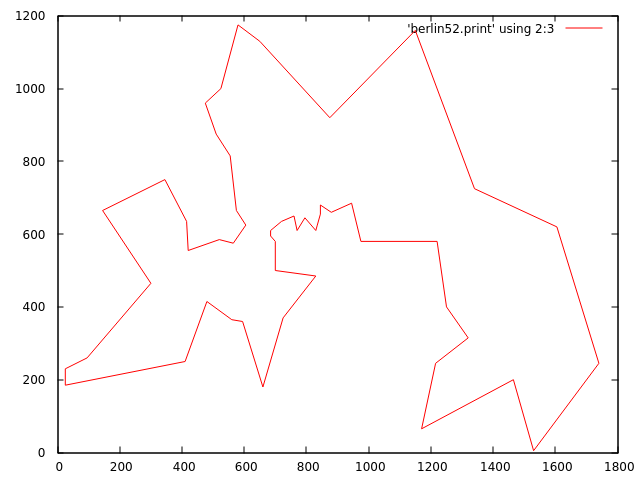
\includegraphics[width=1\textwidth]{berlin52OPT.png}
					
				\end{figure}

\newpage

				\par
				Heurística del vecino más cercano:

				\vspace{5mm}

				\begin{figure}[h]

					\centering
					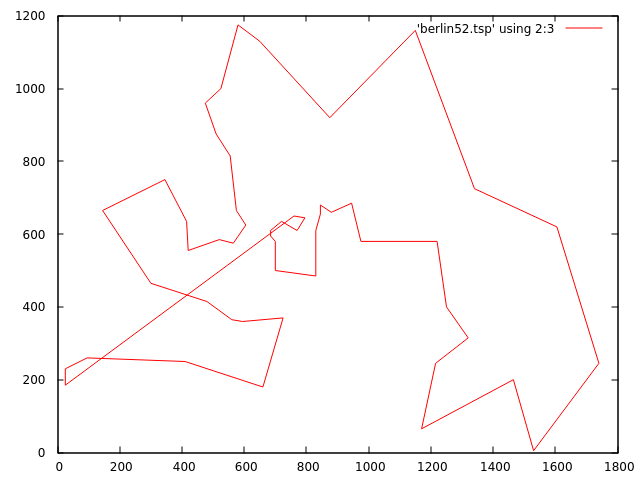
\includegraphics[width=0.7\textwidth]{berlin52VMC.png}
					
				\end{figure}

				\par
				Heurística de la inserción más económica:

				\vspace{5mm}

				\begin{figure}[h]

					\centering
					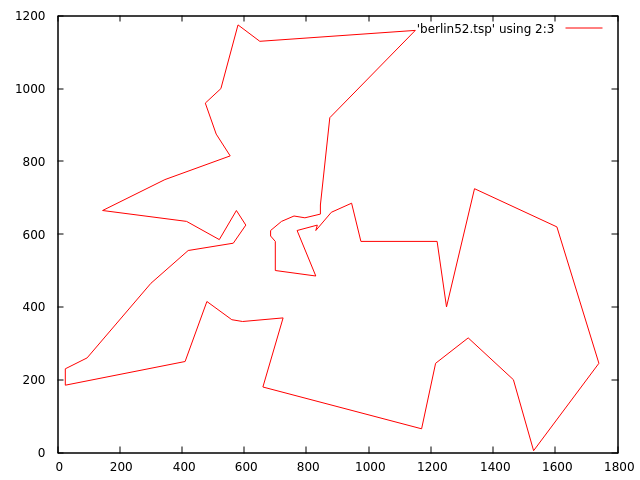
\includegraphics[width=0.7\textwidth]{berlin52IM.png}
					
				\end{figure}

\newpage

				\par
				Heurística de la inserción radial:

				\vspace{5mm}

				\begin{figure}[h]

					\centering
					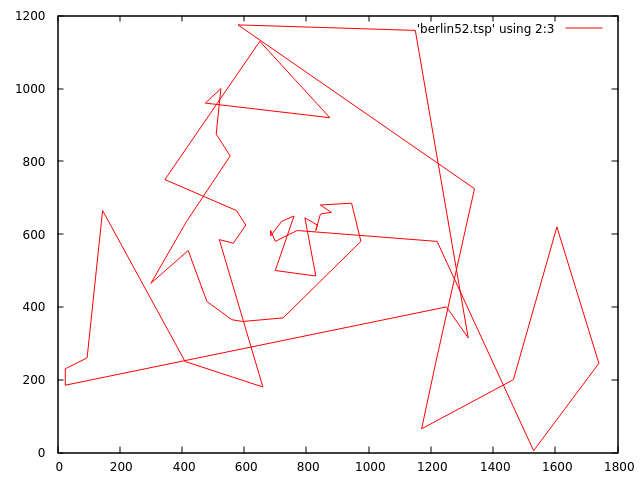
\includegraphics[width=0.7\textwidth]{berlin52IR.png}
					
				\end{figure}

\newpage

			\subsubsection{Instancia \textit{eil51}.}

				\par
				Solución óptima:

				\vspace{5mm}

				\begin{figure}[h]

					\centering
					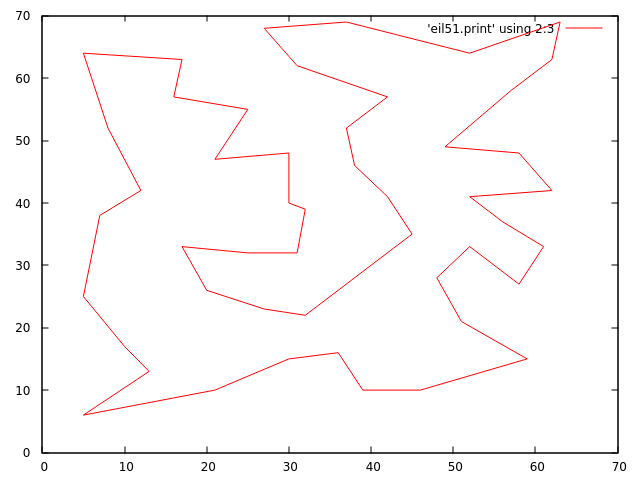
\includegraphics[width=1\textwidth]{eil51OPT.png}
					
				\end{figure}

\newpage

				\par
				Heurística del vecino más cercano:

				\vspace{5mm}

				\begin{figure}[h]

					\centering
					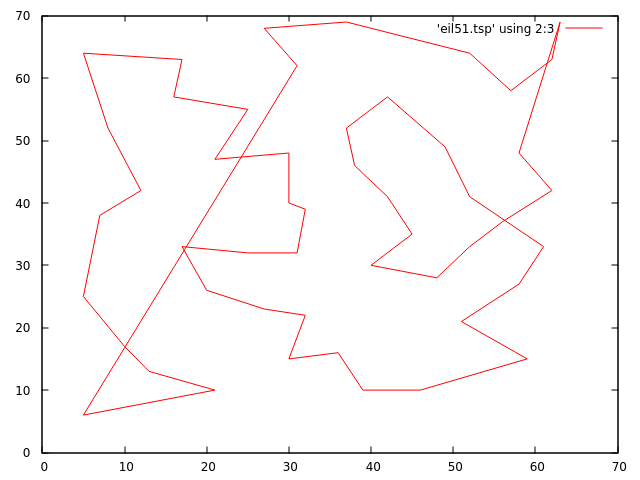
\includegraphics[width=0.7\textwidth]{eil51VMC.png}
					
				\end{figure}

				\par
				Heurística de la inserción más económica:

				\vspace{5mm}

				\begin{figure}[h]

					\centering
					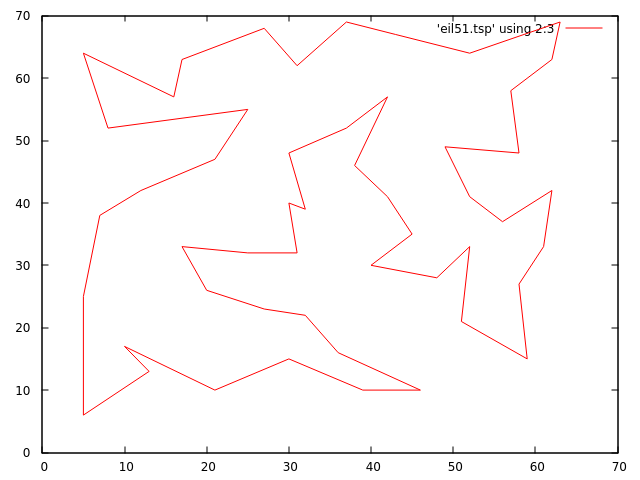
\includegraphics[width=0.7\textwidth]{eil51IM.png}
					
				\end{figure}

\newpage

				\par
				Heurística de la inserción radial:

				\vspace{5mm}

				\begin{figure}[h]

					\centering
					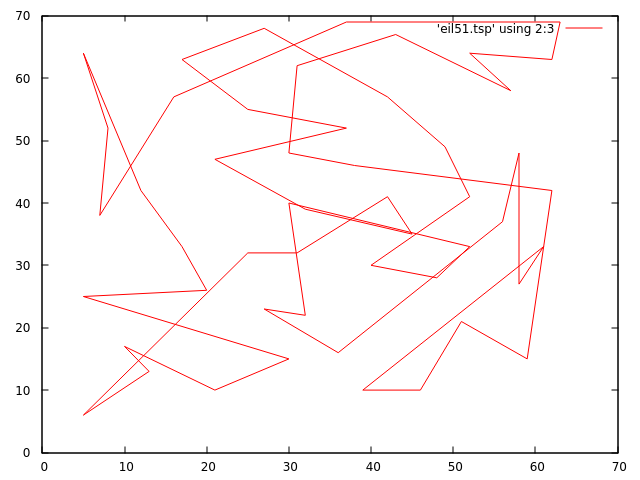
\includegraphics[width=0.7\textwidth]{eil51IR.png}
					
				\end{figure}

\newpage

			\subsubsection{Instancia \textit{gr96}.}

				\par
				Solución óptima:

				\vspace{5mm}

				\begin{figure}[h]

					\centering
					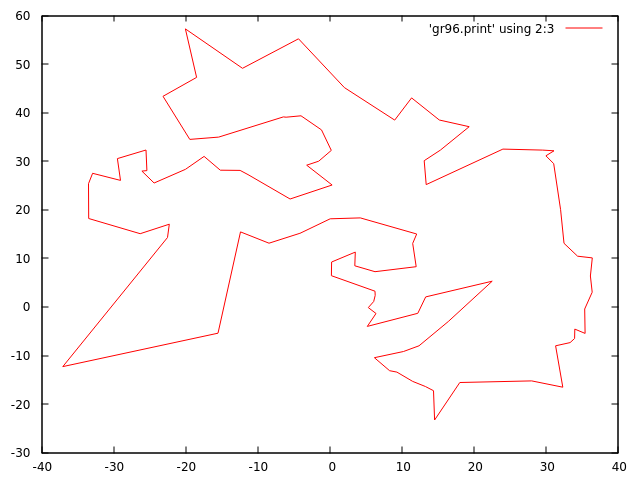
\includegraphics[width=1\textwidth]{gr96OPT.png}
					
				\end{figure}

\newpage

				\par
				Heurística del vecino más cercano:

				\vspace{5mm}

				\begin{figure}[h]

					\centering
					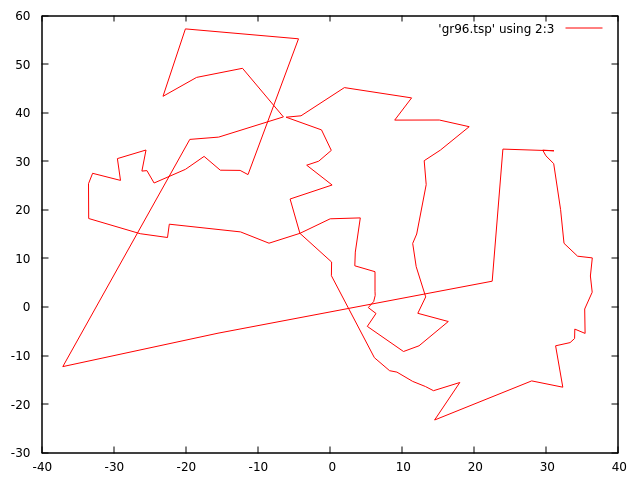
\includegraphics[width=0.7\textwidth]{gr96VMC.png}
					
				\end{figure}

				\par
				Heurística de la inserción más económica:

				\vspace{5mm}

				\begin{figure}[h]

					\centering
					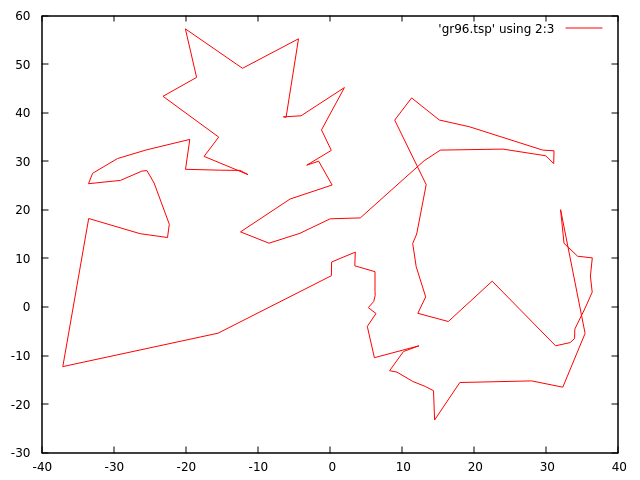
\includegraphics[width=0.7\textwidth]{gr96IM.png}
					
				\end{figure}

\newpage

				\par
				Heurística de la inserción radial:

				\vspace{5mm}

				\begin{figure}[h]

					\centering
					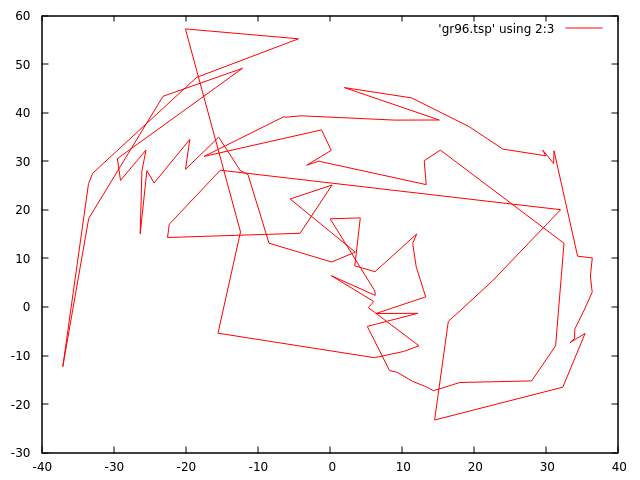
\includegraphics[width=0.7\textwidth]{gr96IR.png}
					
				\end{figure}

\newpage

	\section{Conclusión.}

		\par
		En primer lugar, lo más importante es que la naturaleza de este tipo de algoritmos permite obtener en muchos casos una solución aceptable para el problema del viajante de comercio en muy poco tiempo, pero no la óptima: debido a que es voraz, a veces ignorará en favor de la optimalidad local rutas que un ser humano podría identificar y que a la larga serían más cortas. Se ha sugerido que, si en las etapas finales del algoritmo las elecciones son considerablemente más costosas que al inicio, es bastante probable que haya circuitos mucho mejores.

		\par
		En segundo lugar, debemos tener en cuenta que el método de selección de candidatos es crucial para que el algoritmo \textit{Greedy} ofrezca todo su potencial. Como ha quedado patente a lo largo de este documento, la elección de una buena heurística es lo que marca la diferencia, y más si tenemos en cuenta que las soluciones obtenidas mediante estos algoritmos son frecuentemente empleadas como punto de partida para estrategias más sofisticadas.

\end{document}